\section{Специальный раздел}
\label{sec:special}

\subsection{Требования к разрабатываемой системе}

Требования к разрабатываемой системе представляют собой совокупность параметров и характеристик, которыми должно обладать разрабатываемое приложение для достижения поставленных целей и решения задач. Они определяют функциональность системы, ее поведение, а также условия, необходимые для ее корректной работы. Требования подразделяются на функциональные и нефункциональные.

Функциональные требования описывают специфические функции или действия, которые должна выполнять система. В контексте разрабатываемого приложения для поиска и возврата уянных вещей, это могут быть функции регистрации и авторизации пользователей, поиска утерянных вещей, добавления информации о утерянных вещах, связи между пользователями и системы уведомлений.

Нефункциональные требования определяют качественные характеристики системы, такие как производительность, безопасность, доступность, удобство использования, совместимость, масштабируемость, тестирование и документация.

Требования к разрабатываемой системе играют ключевую роль в процессе разработки приложения. Они служат основой для проектирования, реализации и тестирования системы. Без четко определенных требований невозможно разработать эффективное и надежное приложение, которое будет отвечать потребностям пользователей и бизнес-задачам.

В контексте курсовой работы на тему “Разработка приложения для поиска и возврата утерянных вещей”, требования к разрабатываемой системе позволяют сформулировать и структурировать задачи, которые должно решать приложение, а также определить параметры, необходимые для его успешной работы. Они служат основой для дальнейшего проектирования и разработки приложения, а также для оценки его эффективности и качества после внедрения.

\subsubsection{Функциональные требования}

\begin{enumerate}
	\item Приложение должно предоставлять возможность регистрации и авторизации пользователей.
	\item Приложение должно предоставлять возможность поиска утерянных вещей по различным критериям (например, по типу вещи, по месту утери и т.д.).
	\item Пользователи должны иметь возможность добавлять информацию о утерянных вещах, включая описание, фотографии и место утери.
	\item Приложение должно предоставлять функционал для связи между пользователем, который нашел вещь, и пользователем, который ее потерял.
	\item Приложение должно иметь систему уведомлений, которая будет информировать пользователей о новых найденных вещах, соответствующих их критериям поиска.
\end{enumerate}

В соответствии с требованиями была составлена ER-диаграмма, которая представлена на рис.~\ref{fig:erd}. Пользователь регистрируется посредством OAuth, при этом заполняются таблицы Account и User. Пользователь заполняет свои социальные сети UserSocialNetwork. Пользователь заполняет форму с потерянной или найденной вещью в LostAndFoundItem, и привязывает к карточки вещи соц. сети, по которой с ним можно связаться.

\begin{figure}[htb]
	\centering
	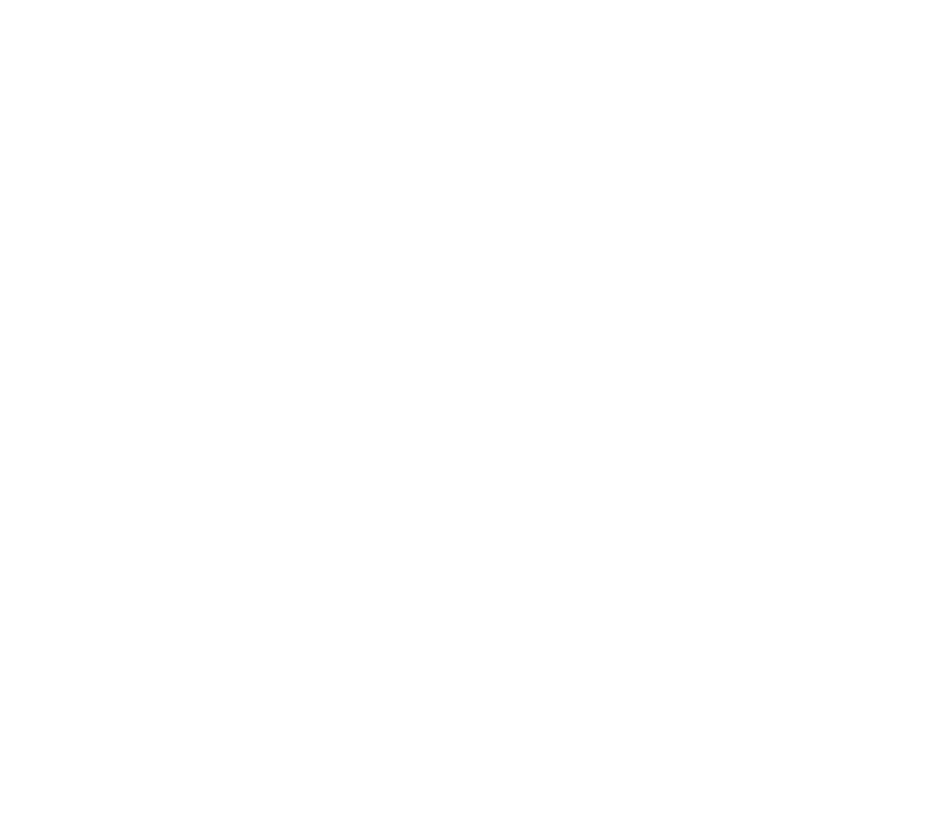
\includegraphics[width=.95\textwidth]{images/erd}
	\parskip=6pt
	\caption{ER-диаграмма системы}
	\label{fig:erd}
\end{figure}

\subsubsection{Нефункциональные требования}

\begin{enumerate}
	\item Приложение должно обеспечивать быстрый поиск и отображение результатов, а также быстрое добавление информации о утерянных вещах.
	\item Все данные пользователей должны быть защищены.
	\item Приложение должно быть доступно для использования 24/7.
	\item Интерфейс приложения должен быть интуитивно понятным и удобным для пользователей разного уровня компьютерной грамотности.
	\item Приложение должно быть совместимо с основными операционными системами (iOS, Android) и браузерами (Chrome, Firefox, Safari, Edge).
	\item Приложение должно быть способно обслуживать большое количество пользователей одновременно без снижения производительности.
	\item Приложение должно быть тщательно протестировано на наличие ошибок и уязвимостей перед запуском.
\end{enumerate}

Клиентское приложение работает в вебе, использует кросс-платформенные технологии (JS, HTML, CSS). Защита пользователя возложено на независимый сервер авторизации.

\subsection{Проектирование модулей автоматизации процессов}

Проектирование модулей автоматизации процессов включает в себя разработку структуры и функционала модулей, которые будут автоматизировать ключевые процессы приложения для поиска и возврата утерянных вещей. В данном случае, ключевыми процессами являются: регистрация и авторизация пользователей, добавление и поиск утерянных вещей, связь между пользователями и система уведомлений.

\begin{figure}[htb]
	\centering
	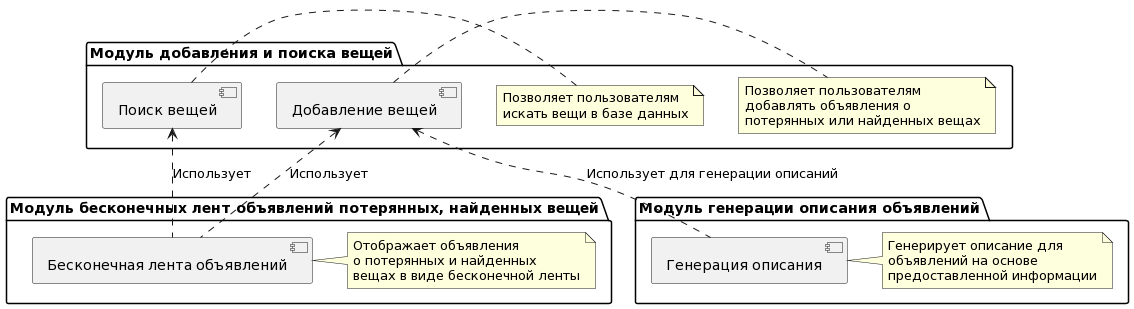
\includegraphics[width=.9\textwidth]{images/full-diagram.png}
	\parskip=6pt
	\caption{Диаграмма компонентов системы}
	\label{fig:агддВшфпкфь}
\end{figure}

\begin{comment}
@startuml
package "Модуль бесконечных лент объявлений потерянных, найденных вещей" {
	[Бесконечная лента объявлений] as InfiniteScroll
	note right of InfiniteScroll : Отображает объявления\nо потерянных и найденных\nвещах в виде бесконечной ленты
}

package "Модуль добавления и поиска вещей" {
	[Добавление вещей] as AddItems
	[Поиск вещей] as SearchItems
	note right of AddItems : Позволяет пользователям\nдобавлять объявления о\nпотерянных или найденных вещах
	note right of SearchItems : Позволяет пользователям\nискать вещи в базе данных
}

package "Модуль генерации описания объявлений" {
	[Генерация описания] as DescriptionGeneration
	note right of DescriptionGeneration : Генерирует описание для\nобъявлений на основе\nпредоставленной информации
}

'Relations
InfiniteScroll .up.> AddItems : Использует
InfiniteScroll .up.> SearchItems : Использует
DescriptionGeneration .up.> AddItems : Использует для генерации описаний
@enduml
\end{comment}

\subsubsection{Модуль регистрации и авторизации пользователей}

Этот модуль предназначен для создания и поддержки учетных записей пользователей. Он должен включать функции регистрации, авторизации через сервер посредника (сервер авторизации РТУ МИРЭА).


\begin{figure}[htb]
	\centering
	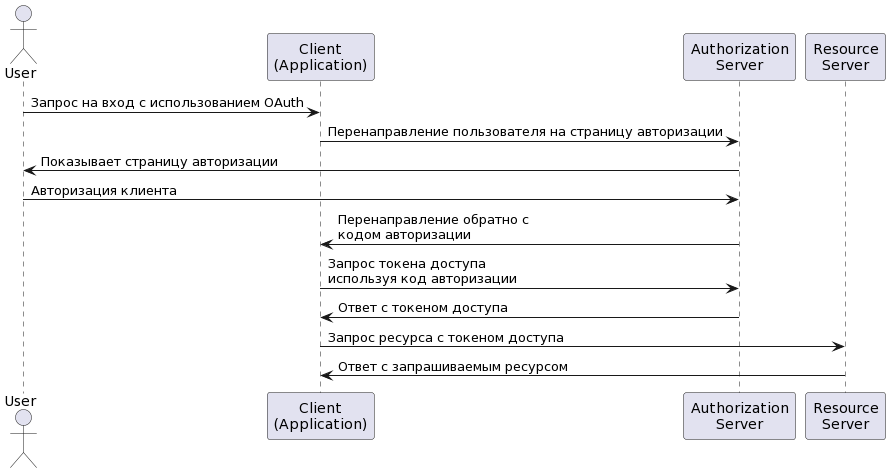
\includegraphics[width=.9\textwidth]{images/registation-diagram.png}
	\parskip=6pt
	\caption{Диаграмма последовательностей авторизации}
	\label{fig:authDiagram}
\end{figure}

\begin{comment}
@startuml
actor User as user
participant "Client\n(Application)" as client
participant "Authorization\nServer" as auth
participant "Resource\nServer" as resource

user -> client: Запрос на вход с использованием OAuth
client -> auth: Перенаправление пользователя на страницу авторизации
auth -> user: Показывает страницу авторизации
user -> auth: Авторизация клиента
auth -> client: Перенаправление обратно с\nкодом авторизации
client -> auth: Запрос токена доступа\nиспользуя код авторизации
auth -> client: Ответ с токеном доступа
client -> resource: Запрос ресурса с токеном доступа
resource -> client: Ответ с запрашиваемым ресурсом
@enduml
\end{comment}


\subsubsection{Модуль бесконечных лент объявлений потерянных, найденных вещей}

Модуль бесконечных лент объявлений представляет собой ключевой элемент приложения для поиска и возврата утерянных вещей. Он предназначен для отображения объявлений о потерянных и найденных вещах в формате бесконечной ленты, обеспечивая пользователю удобный и непрерывный доступ к информации.

\begin{figure}[htb]
	\centering
	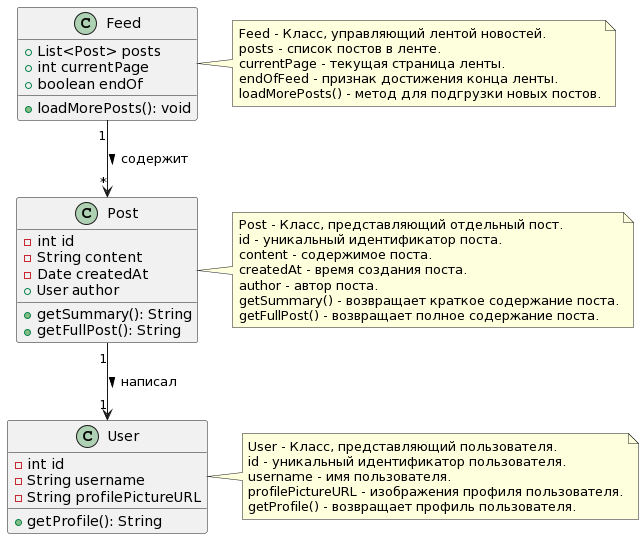
\includegraphics[width=.9\textwidth]{images/feed-diagram.png}
	\parskip=6pt
	\caption{Диаграмма классов бесконечной ленты}
	\label{fig:feedDiagram}
\end{figure}

\begin{comment}
@startuml
class Feed {
	+List<Post> posts
	+int currentPage
	+boolean endOf
	+loadMorePosts(): void
}

class Post {
	-int id
	-String content
	-Date createdAt
	+User author
	+getSummary(): String
	+getFullPost(): String
}

class User {
	-int id
	-String username
	-String profilePictureURL
	+getProfile(): String
}

Feed "1" --> "*" Post : содержит >
Post "1" --> "1" User : написал >

note right of Feed
Feed - Класс, управляющий лентой новостей.
posts - список постов в ленте.
currentPage - текущая страница ленты.
endOfFeed - признак достижения конца ленты.
loadMorePosts() - метод для подгрузки новых постов.
end note

note right of Post
Post - Класс, представляющий отдельный пост.
id - уникальный идентификатор поста.
content - содержимое поста.
createdAt - время создания поста.
author - автор поста.
getSummary() - возвращает краткое содержание поста.
getFullPost() - возвращает полное содержание поста.
end note

note right of User
User - Класс, представляющий пользователя.
id - уникальный идентификатор пользователя.
username - имя пользователя.
profilePictureURL - изображения профиля пользователя.
getProfile() - возвращает профиль пользователя.
end note
@enduml
\end{comment}

\subsubsection{Модуль добавления и поиска вещей}

Этот модуль отвечает за добавление информации о утерянных вещах в базу данных и поиск по этой базе. Он должен предоставлять пользователю возможность добавлять описание, фотографии и место утери вещи, а также осуществлять поиск по различным критериям.

\begin{figure}[htb]
	\centering
	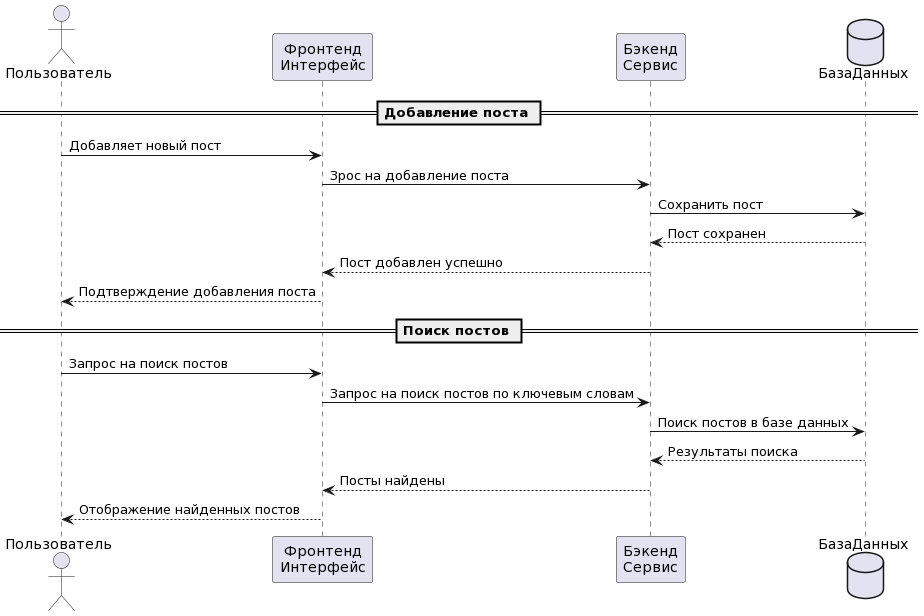
\includegraphics[width=.9\textwidth]{images/seach-diagram.png}
	\parskip=6pt
	\caption{Диаграмма последовательностей добавления и поиска вещей}
	\label{fig:searchDiagram}
\end{figure}

\begin{comment}
@startuml
actor Пользователь as User
participant "Фронтенд\nИнтерфейс" as Frontend
participant "Бэкенд\nСервис" as Backend
database БазаДанных as Database

== Добавление поста ==
User -> Frontend : Добавляет новый пост
Frontend -> Backend : Запрос на добавление поста
Backend -> Database : Сохранить пост
Database --> Backend : Пост сохранен
Backend --> Frontend : Пост добавлен успешно
Frontend --> User : Подтверждение добавления поста

== Поиск постов ==
User -> Frontend : Запрос на поиск постов
Frontend -> Backend : Запрос на поиск постов по ключевым словам
Backend -> Database : Поиск постов в базе данных
Database --> Backend : Результаты поиска
Backend --> Frontend : Посты найдены
Frontend --> User : Отображение найденных постов
@enduml
\end{comment}

\begin{figure}[htb]
	\centering
	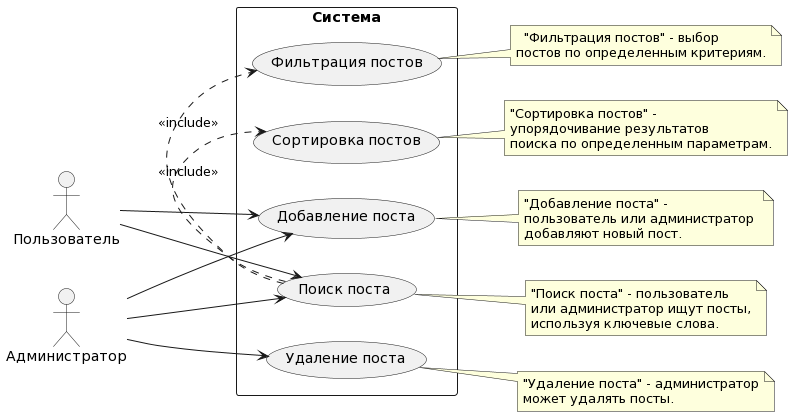
\includegraphics[width=.9\textwidth]{images/seach-diagram-2.png}
	\parskip=6pt
	\caption{Диаграмма вариантов использования добавления и поиска вещей}
	\label{fig:searchDiagram2}
\end{figure}

\begin{comment}
@startuml
left to right direction
actor Пользователь
actor Администратор

rectangle Система {
	Пользователь --> (Добавление поста)
	Пользователь --> (Поиск поста)
	Администратор --> (Добавление поста)
	Администратор --> (Поиск поста)
	Администратор --> (Удаление поста)
	(Поиск поста) .> (Фильтрация постов) : <<include>>
	(Поиск поста) .> (Сортировка постов) : <<include>>
}

note right of (Добавление поста)
"Добавление поста" - 
пользователь или администратор 
добавляют новый пост.
end note

note right of (Поиск поста)
"Поиск поста" - пользователь 
или администратор ищут посты,
используя ключевые слова.
end note

note right of (Удаление поста)
"Удаление поста" - администратор
может удалять посты.
end note

note right of (Фильтрация постов)
"Фильтрация постов" - выбор
постов по определенным критериям.
end note

note right of (Сортировка постов)
"Сортировка постов" - 
упорядочивание результатов 
поиска по определенным параметрам.
end note
@enduml
\end{comment}

\subsubsection{Модуль генерации описания объявлений}

Модуль генерации описания объявлений является важным компонентом приложения для поиска и возврата утерянных вещей. Он предназначен для автоматического создания описаний объявлений на основе введенных пользователем данных, что облегчает процесс создания объявлений и повышает их качество.

\begin{figure}[htb]
	\centering
	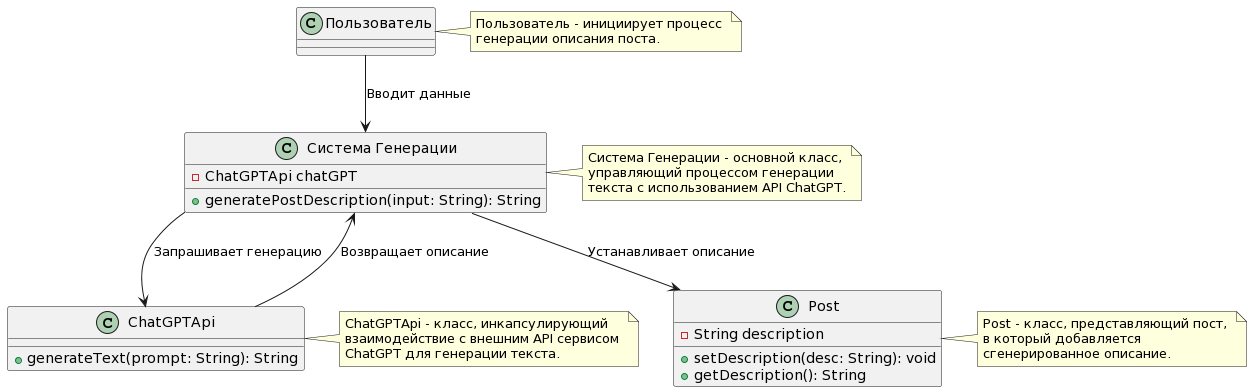
\includegraphics[width=.95\textwidth]{images/generating-diagram.png}
	\parskip=6pt
	\caption{Диаграмма классов генеарации описания вещей}
	\label{fig:generatingDiagram}
\end{figure}

\begin{comment}
@startuml
class "Пользователь" as User {
}

class "Система Генерации" {
	-ChatGPTApi chatGPT
	+generatePostDescription(input: String): String
}

class "ChatGPTApi" {
	+generateText(prompt: String): String
}

class "Post" {
	-String description
	+setDescription(desc: String): void
	+getDescription(): String
}

User --> "Система Генерации" : Вводит данные
"Система Генерации" --> ChatGPTApi : Запрашивает генерацию
ChatGPTApi --> "Система Генерации" : Возвращает описание
"Система Генерации" --> Post : Устанавливает описание

note right of User
Пользователь - инициирует процесс 
генерации описания поста.
end note

note right of "Система Генерации"
Система Генерации - основной класс, 
управляющий процессом генерации 
текста с использованием API ChatGPT.
end note

note right of ChatGPTApi
ChatGPTApi - класс, инкапсулирующий 
взаимодействие с внешним API сервисом 
ChatGPT для генерации текста.
end note

note right of Post
Post - класс, представляющий пост, 
в который добавляется 
сгенерированное описание.
end note
@enduml
\end{comment}

\subsection*{Вывод по разделу}

Проектирование модулей автоматизации процессов является важным этапом в разработке приложения для поиска и возврата утерянных вещей. Каждый из модулей, включая модуль регистрации и авторизации пользователей, модуль бесконечных лент объявлений, модуль добавления и поиска утерянных вещей и модуль генерации описания объявлений, играет свою уникальную роль в обеспечении функциональности приложения.

Каждый из этих модулей важен для обеспечения удобства использования приложения, и их совместная работа позволяет создать надежное и функциональное приложение для поиска и возврата утерянных вещей.